\documentclass{beamer}

\usepackage{amsmath, amssymb}
\usepackage{tikz-cd}
\usepackage{xcolor}
\usepackage{graphicx}

\title{MAT434: Theory of Mathematical Statistics}
\author{\textbf{Miraj Samarakkody}}
\institute{Tougaloo College}
\date{03/28/2025}

\begin{document}

\begin{frame}
    \titlepage
\end{frame}



\begin{frame}{}
    \begin{center}
        \Huge{2.3 Functions of a Random Variable}
    \end{center}

\end{frame}






    


\begin{frame}
    \frametitle{Proposition C}
    \begin{block}{Proposition}
        Let \(Z=F(X)\); then \(Z\) has a uniform distribution of \([0,1]\).
    \end{block}
    \begin{block}{Proof:}
        
    \end{block}


    

\end{frame}

\begin{frame}
    \frametitle{Proposition D}

    \begin{block}{Proposition}
        Let \(U\) be uniform on \([0,1]\), and let \(X = F^{-1}(U)\). Then the cdf of \(X\) is \(F\). 
    \end{block}
    \begin{block}{Proof:}
        
    \end{block}

\end{frame}


\begin{frame}{Chapter 3}
 \Huge{Joint Distributions}
\end{frame}

\begin{frame}
    \frametitle{3.1 Introduction}

    \begin{block}{Definition}
        Two or more random variables defined on the same sample space are said to have a joint probability structure.
    \end{block}\pause

    \begin{block}{Applications}
        \begin{itemize}
            \item In ecological studies. For an example when we count several species, one species is often the prey of another. i.e. the number of predators will be related to the number of prey.  \pause 
            \item The joint probability distribution of the \(x\), \(y\), and \(z\) components of wind velocity can be experimentally measured in studies of atmospheric turbulence. \pause 
            \item The joint distribution of the values of various physiological variables in a population of patients is often of interest in medical studies. \pause
            \item A model for the joint distribution of age and length in a population of fish can be used to estimate the age distribution from the length distribution.
        \end{itemize}
    \end{block}

\end{frame}


\begin{frame}{Introduction}
    The joint behavior of two random variables, \(X\) and \(Y\), is determined by the cumulative distribution function \[F(x,y)= P(X \leq x, Y \leq y)\] regardless of whether \(X\) and \(Y\) are continuous or discrete. \\ \pause 
    \vspace{0.1in}
    The cdf gives the probability that the point \((X,Y)\) beliongs to a semi-infinite rectangle in the plane. 
    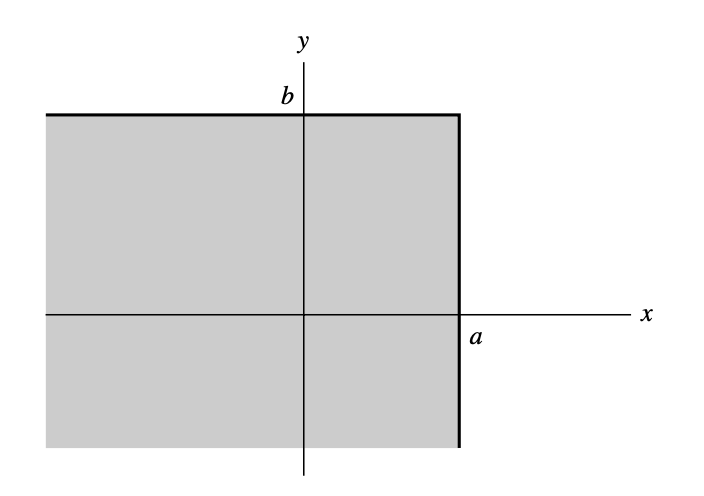
\includegraphics[scale=0.5]{Figures/Figure_5.png}
\end{frame}

\begin{frame}{Introduction}
    The probability that \((X,Y)\) belongs to a rectangle if \begin{align*}
        P(x_1 \leq X \leq x_2, y_1 \leq Y \leq y_2) &= F(x_2,y_2) - F(x_2,y_1) \notag \\
        &\quad - F(x_1, y_2) + F(x_1,y_1)
    \end{align*}
    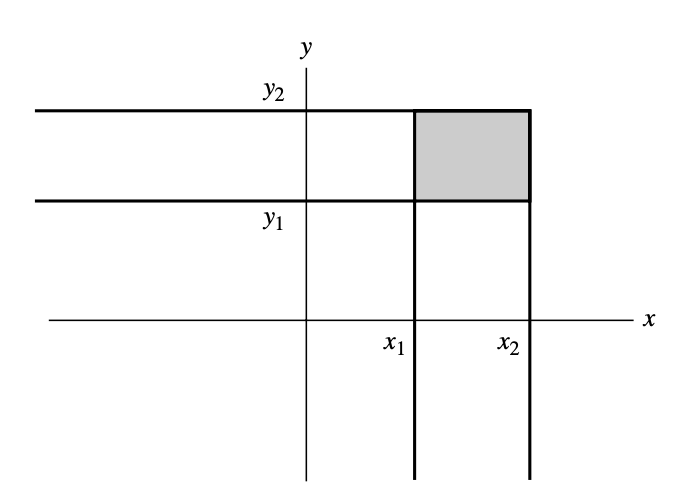
\includegraphics[scale=0.5]{Figures/Figure_6.png}
\end{frame}

\begin{frame}{Discrete Random Variables}
    Suppose that \(X\) and \(Y\) are discrete random variables defined on the same sample space and that they take on values \(x_1,x_2, \dots\), and \(y_1,y_2, \dots\) respectively. \\ \pause
    \vspace{0.1in}

    Their \textbf{joint frequency function} \(p(x,y)\) is \[
    p(x_i, y_j) =P(X=x_i, Y=y_j)
    \]
\end{frame}

\begin{frame}{Example}
    A fair coin is tossed three times and let \(X\) denote the number of heads on the first toss and \(Y\) the total number of heads. Find joint frequency function of \(X\) and \(Y\).  \\ \pause
    \vspace{0.2in}
    Find the frequency function of \(Y\) \((p_Y)\) from the joint frequency function. \\ \pause
    \vspace{0.2in}
    The \(p_Y\) is called the \textbf{marginal frequency function} of \(Y\). 
\end{frame}

\begin{frame}{Marginal Frequency Function}
Let \(X\) and \(Y\) are discrete random variables defined on the same sample space. The marginal function of \(X\) can be written as 
\[p_X(x)= \sum_i p(x,y_i)\] In the similary way, we can write the marginal frequency function for \(Y\).
\end{frame}


\end{document}